\apendice{Documentación de usuario}

\section{Introducción}

%Se recomienda a los usuarios seguir cuidadosamente cada sección de este manual para garantizar una implementación exitosa y para aprovechar todas las capacidades que ofrece el sistema IoT de monitorización de invernaderos. 
Este documento está diseñado para facilitar la comprensión y el uso del sistema, contribuyendo así a una experiencia de usuario satisfactoria y a la consecución de los objetivos de monitorización de cultivos de cannabis medicinal de manera eficaz y económica.

%\section{Requisitos de usuarios}

\section{Instalación Física}
Se tiene que instalar el firmware en la Raspberry Pi Pico W para que podamos programarlo mediante Micropython.
Primero descargamos el firmware de Micropython desde su página oficial~\cite{misc:MicropythonFirmware}.

Para fines prácticos nombraremos al firmware descargado: \textbf{rp2-pico.uf2}.

\begin{figure}[h]
\centering
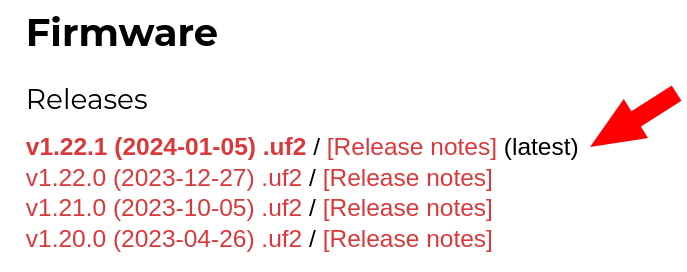
\includegraphics[width=0.7\textwidth]{img/herramientas/micropython_firmware.png}
\caption{Descargar el firmware más reciente.}
\end{figure}

Conectar el puerto usb de la Raspberry Pi Pico W manteniendo presionado el botón \textbf{BOOTSEL}.

\begin{figure}[h]
\centering
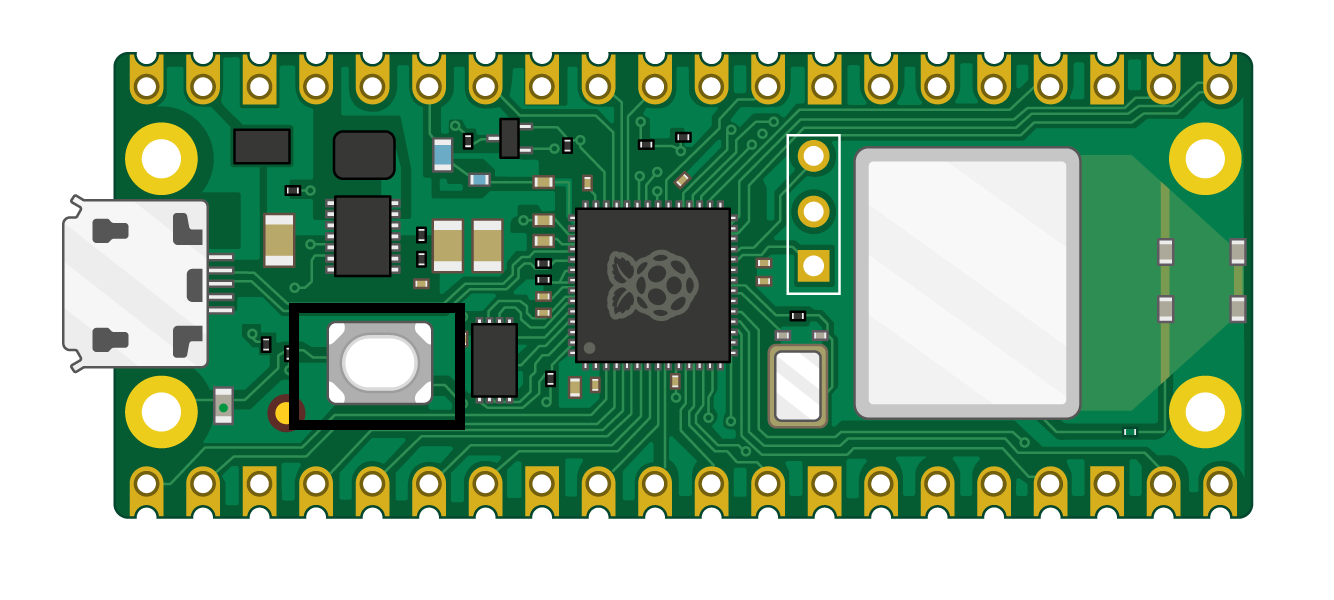
\includegraphics[width=1\textwidth]{img/herramientas/rpipicow_boton.png}
\caption{Conectar usb manteniendo presionado.}
\end{figure}

Se ha creado un script en bash al que llamamos \textbf{instaladorFirmware.sh}. La ejecución de este permitirá instalar el firmware de Micropython en la Raspberry Pi Pico W.


\begin{lstlisting}[language=sh, firstnumber=0, basicstyle=\normalsize, caption={Script en bash para instalar el firmware Micropython.}] 
puerto=$(sudo dmesg | tail | grep -o 'sd[b-z]1')
sudo mkdir /mnt/pico
sudo mount /dev/$puerto /mnt/pico
sudo cp rp2-pico.uf2 /mnt/pico
sudo sync
\end{lstlisting}

Tener presente que el archivo \textbf{instaladorFirmware.sh} y el firmware descargado, deben estar en el mismo directorio.

\begin{lstlisting}[language=sh, firstnumber=0, basicstyle=\normalsize, caption={Comando para dar permisos de ejecución.}] 
sudo chmod +x instaladorFirmware.sh\end{lstlisting}

\begin{lstlisting}[language=sh, firstnumber=0, basicstyle=\normalsize, caption={Comando para ejecutar el instalador de Firmware.}] 
sudo ./instaladorFirmware.sh\end{lstlisting}


Usando el IDE Thonny~\cite{misc:Thonny} y con Micropython vamos a poder programar el hardware. Lo podemos descargar e instalar desde su pagina oficial~\cite{misc:Thonny}.

Tenemos que hacer unas configuraciones simples antes de poder usar el IDE Thonny con Micropython en nuestra Raspberry Pi Pico W.

Hacemos clic en \textbf{Run/Configure interpreter}.

\begin{figure}[h]
	\centering
	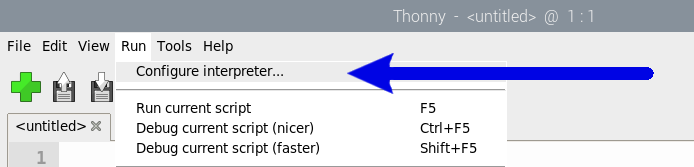
\includegraphics[width=0.9\textwidth]{img/desarrollo/thonny_interpreter.png}
	\caption{Abrimos el configurador del interpreter.}
\end{figure}

Seleccionamos que usaremos \textbf{Micropython} para Raspberry Pi Pico y seleccionamos el puerto que corresponde su conexión por usb.

\begin{figure}[h]
	\centering
	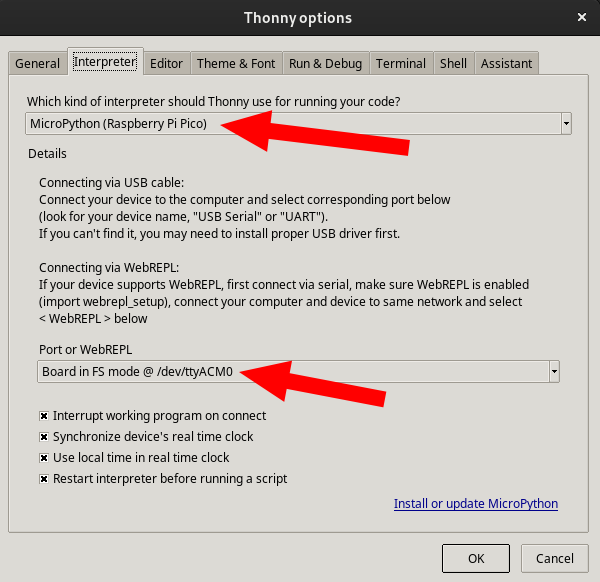
\includegraphics[width=0.9\textwidth]{img/desarrollo/thonny_seleccionInterpreter.png}
	\caption{Habilitamos Thonny para Micropython.}
\end{figure}

Usar los archivos del directorio \textbf{Hardware} para guardarlos en la Raspberry Pi Pico W usando el IDE Thonny.

\begin{figure}[h]
	\centering
	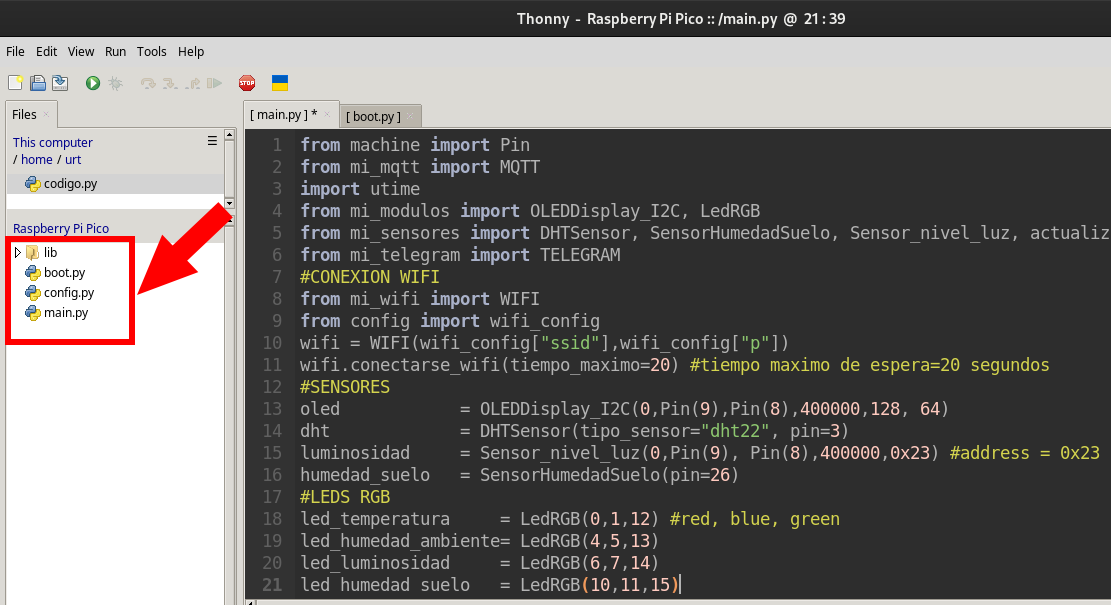
\includegraphics[width=0.9\textwidth]{img/desarrollo/thonny_archivosNecesarios.png}
	\caption{Archivos necesarios para ejecutar en el hardware.}
\end{figure}


\begin{figure}[h]
	\centering
	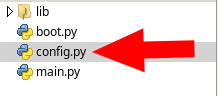
\includegraphics[width=0.4\textwidth]{img/desarrollo/thonny_config.png}
	\caption{Archivo de configuración en Micropython.}
\end{figure}

Modificamos el archivo \textbf{config.py} con nuestras credenciales.

\begin{lstlisting}[language=sh, firstnumber=0, basicstyle=\normalsize, caption={Configurar SSID y clave wifi.}] 
wifi_config = {
    'ssid':'SSID_WIFI',
    'p':'TU_PASSWORD_WIFI'
}\end{lstlisting}



\begin{lstlisting}[language=sh, firstnumber=0, basicstyle=\normalsize, caption={Configución de bot de Telegram.}] 
utelegram_config = {
    'token': 'BOT_TOKEN_TELEGRAM',
    'chat_id': 'BOT_CHAT_ID'
}
\end{lstlisting}

\begin{lstlisting}[language=sh, firstnumber=0, basicstyle=\normalsize, caption={Configuración de umbrales para los sensores.}] 
umbrales_sensores = {
    'TEMPERATURA_MINIMA': 30,
    'HUMEDAD_MINIMA': 30,
    'LUMINOSIDAD_MINIMA': 30,
    'HUMEDAD_SUELO_MINIMA': 20,
    'TEMPERATURA_MAXIMA': 35,
    'HUMEDAD_MAXIMA': 70,
    'LUMINOSIDAD_MAXIMA': 150,
    'HUMEDAD_SUELO_MAXIMA': 80
}
\end{lstlisting}

\begin{lstlisting}[language=sh, firstnumber=0, basicstyle=\normalsize, caption={Configuración MQTT.}] 
mqtt_config = {
    'server': '1.39.4.38', #IP DE TU SERVIDOR LAMP
    'port': 1883, #PUERTO USADO POR MQTT
    'topic_pub': 'invernadero/sensores',
    'topic_sub': 'invernadero/ordenes',
    'topic_umb': 'invernadero/umbrales',
    'client_id_pub': 'TFG_UBU_mqtt_id_pub',
    'client_id_sub': 'TFG_UBU_mqtt_id_sub',
    'client_id_umb': 'TFG_UBU_mqtt_id_umb'
}
\end{lstlisting}

\begin{lstlisting}[language=sh, firstnumber=0, basicstyle=\normalsize, caption={Configuración Wlan para usar ip fija.}] 
wlan_config = {
    'ip':'192.168.1.232',
    'mask':'255.255.255.0',
    'gateway':'192.168.1.1',
    'dns':'8.8.8.8' 
}
\end{lstlisting}

Una vez que haz completado las credenciales ya puedes desconectar y volver a conectar la Rapsberry Pi Pico W, al arrancar automáticamente se ejecutará la programación ya establecida.

Solo volverás a usar el IDE Thonny si quieres cambiar algo en el código o en el archivo de configuración.

Ahora procedemos a hacer las conexiones en el hardware.

Solo comprobar que todas las conexiones sean coherentes a la imagen.

\begin{figure}[h]
\centering
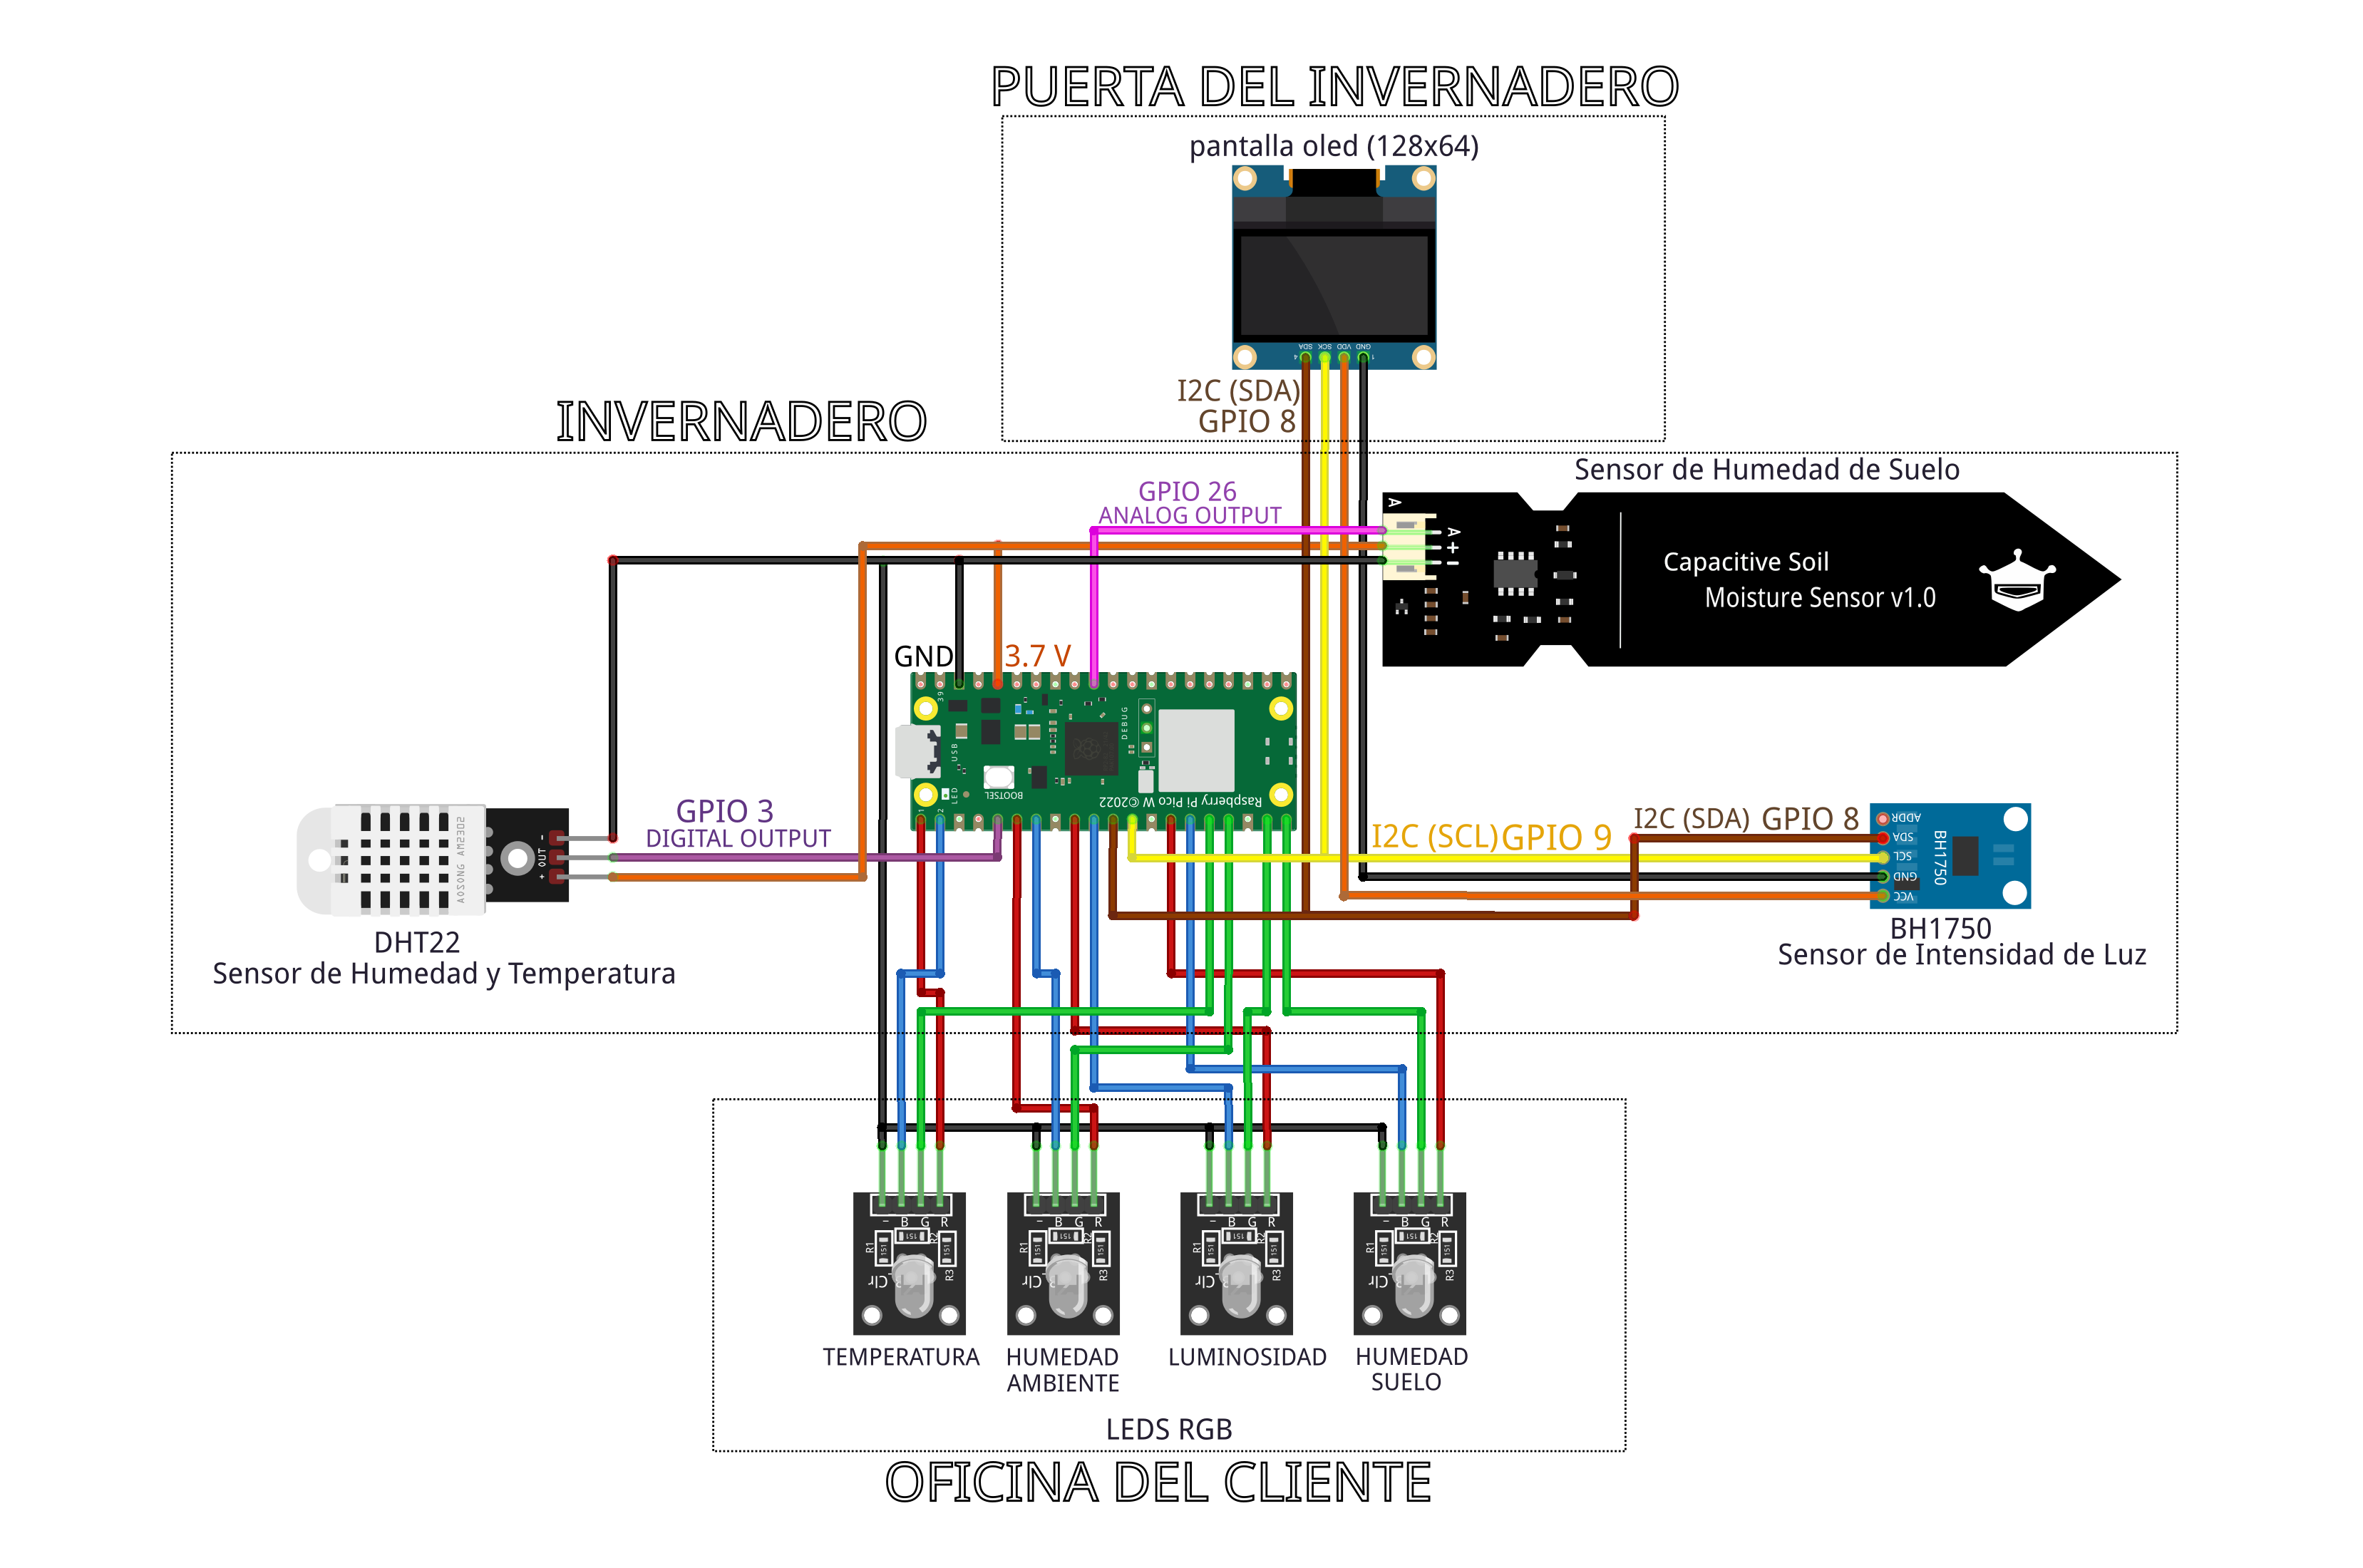
\includegraphics[width=1\textwidth]{img/diagramas/conexiones.png}
\caption{Conexiones del hardware para el cliente.}
\end{figure}


\section{Instalación del software}

\subsection{Servidor LAMP}
Se ha creado un script en bash para hacer las instalaciones automáticamente al que se ha nombrado \textbf{InstaladorServidor.sh}.

\begin{lstlisting}[language=sh, firstnumber=0, basicstyle=\normalsize, caption={Damos permisos de ejecución a \textbf{InstaladorServidor.sh}.}] 
sudo chmod +x InstaladorServidor.sh
\end{lstlisting}

\begin{lstlisting}[language=sh, firstnumber=0, basicstyle=\normalsize, caption={Contenido de \textbf{InstaladorServidor.sh}.}] 
sudo apt install apache2
sudo apt install mysql-server
sudo apt install php
sudo apt install ssh
sudo apt install phpmyadmin
sudo apt install vsftpd
sudo apt install ufw 
sudo apt install nodejs
sudo apt install pm2
sudo apt install npm
sudo apt install express
sudo apt install mosquitto 
\end{lstlisting}

\begin{lstlisting}[language=sh, firstnumber=0, basicstyle=\normalsize, caption={Ejecutamos \textbf{InstaladorServidor.sh}.}] 
sudo ./InstaladorServidor.sh
\end{lstlisting}

\subsection{Creación de base de datos}
\begin{lstlisting}[language=sh, firstnumber=0, basicstyle=\normalsize, caption={Comando para acceder a Mysql.}] 
sudo mysql\end{lstlisting}

\begin{lstlisting}[language=sh, firstnumber=0, basicstyle=\normalsize, caption={Comandos Mysql para crear Database \textbf{TFG\_UBU}.}] 
CREATE DATABASE TFG_UBU;
CREATE USER 'joseluis'@'%' IDENTIFIED BY 'Mipassword';
GRANT ALL ON TFG_UBU.* TO 'joseluis'@'%';
use TFG_UBU;
\end{lstlisting}


\begin{lstlisting}[language=sh, firstnumber=0, basicstyle=\normalsize, caption={Comandos Mysql para crear tabla \textbf{umbrales}.}] 
CREATE TABLE `umbrales` (
  `temperatura_minima` float NOT NULL,
  `temperatura_maxima` float NOT NULL,
  `humedad_ambiente_minima` float NOT NULL,
  `humedad_ambiente_maxima` float NOT NULL,
  `luminosidad_minima` float NOT NULL,
  `luminosidad_maxima` float NOT NULL,
  `humedad_suelo_minima` float NOT NULL,
  `humedad_suelo_maxima` float NOT NULL,
  `fecha_actualizacion` timestamp 
  NULL DEFAULT CURRENT_TIMESTAMP 
  ON UPDATE CURRENT_TIMESTAMP
) ENGINE=InnoDB DEFAULT CHARSET=utf8mb4;
INSERT INTO `umbrales` (
`temperatura_minima`, `temperatura_maxima`, 
`humedad_ambiente_minima`, `humedad_ambiente_maxima`, 
`luminosidad_minima`, `luminosidad_maxima`, 
`humedad_suelo_minima`, `humedad_suelo_maxima`) VALUES
(30, 35, 30, 70, 30, 150, 20, 80);
\end{lstlisting}

\begin{lstlisting}[language=sh, firstnumber=0, basicstyle=\normalsize, caption={Comandos Mysql para crear tabla \textbf{sensores}.}] 
CREATE TABLE `sensores` (
  `id` int NOT NULL AUTO_INCREMENT,
  `fecha` date DEFAULT NULL,
  `hora` time DEFAULT NULL,
  `temperatura` decimal(4,2) DEFAULT NULL,
  `humedad` decimal(4,2) DEFAULT NULL,
  `intensidad_luz` decimal(4,2) DEFAULT NULL,
  `humedad_suelo` decimal(4,2) DEFAULT NULL,
  PRIMARY KEY (`id`)
) ENGINE=InnoDB DEFAULT CHARSET=utf8mb4;
\end{lstlisting}


\subsection{dashboard}

\begin{lstlisting}[language=sh, firstnumber=0, basicstyle=\normalsize, caption={Instalaciones necesarias.}] 
npm install express
npm install socket.io
\end{lstlisting}

Respecto al archivo \textbf{servers.js} debemos configurar respecto a la base de datos creada en el servidor LAMP:

\begin{lstlisting}[language=cpp, firstnumber=0, basicstyle=\normalsize, caption={Configuración de base de datos.}] 
const dbConfig = {
    host: 'localhost',
    port: 3307, // Puerto especificado aquí
    user: 'joseluis',
    password: 'TuPassword',
    database: 'TFG_UBU'
};
\end{lstlisting}

Solo se ejecuta una vez y siempre va a estar ejecutándose, incluso si se reinicia el servidor.

\begin{lstlisting}[language=sh, firstnumber=0, basicstyle=\normalsize, caption={Ejecución.}] 
mp2 start servers.js --name "dashboard"
\end{lstlisting}

\subsection{InverIoT}
Solo ejecutar el instalador \textbf{Instalador - InverIoT - v2.2.exe}.

\section{Manual del usuario}

Una vez todo está instalado y configurado ya puedes interactuar con las diferentes partes del proyecto.

\subsection{Hardware}
Solo conectar la Raspberry Pi Pico a una fuente de energía y está operativo.

\begin{figure}[h]
\centering
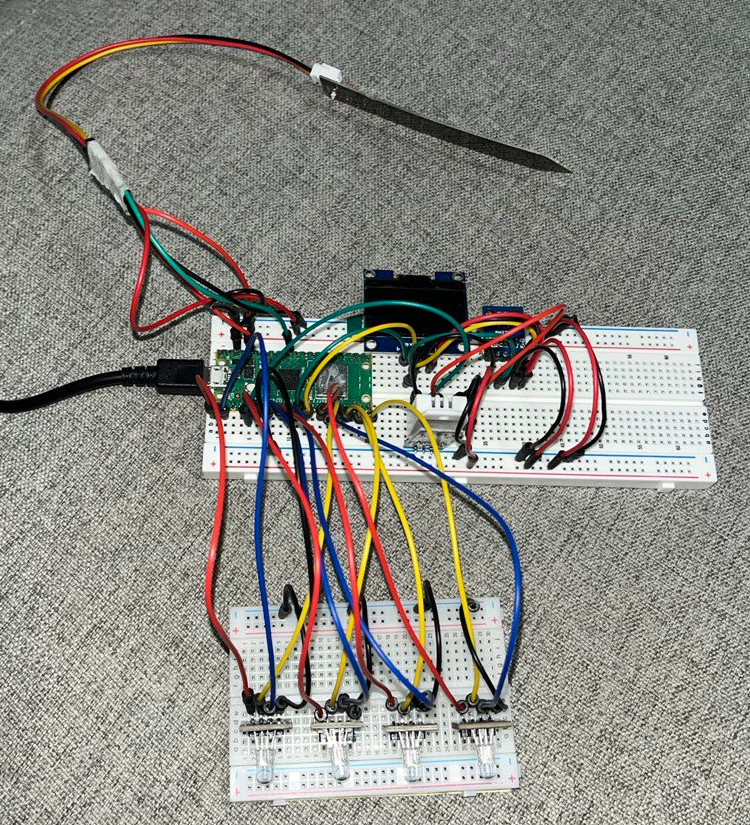
\includegraphics[width=0.9\textwidth]{img/fotos/conexiones_real.png}
\caption{Foto real de las conexiones.}
\end{figure}

Clavar el sensor de humedad de suelo en el punto que se desea monitorear.

\begin{figure}[h]
\centering
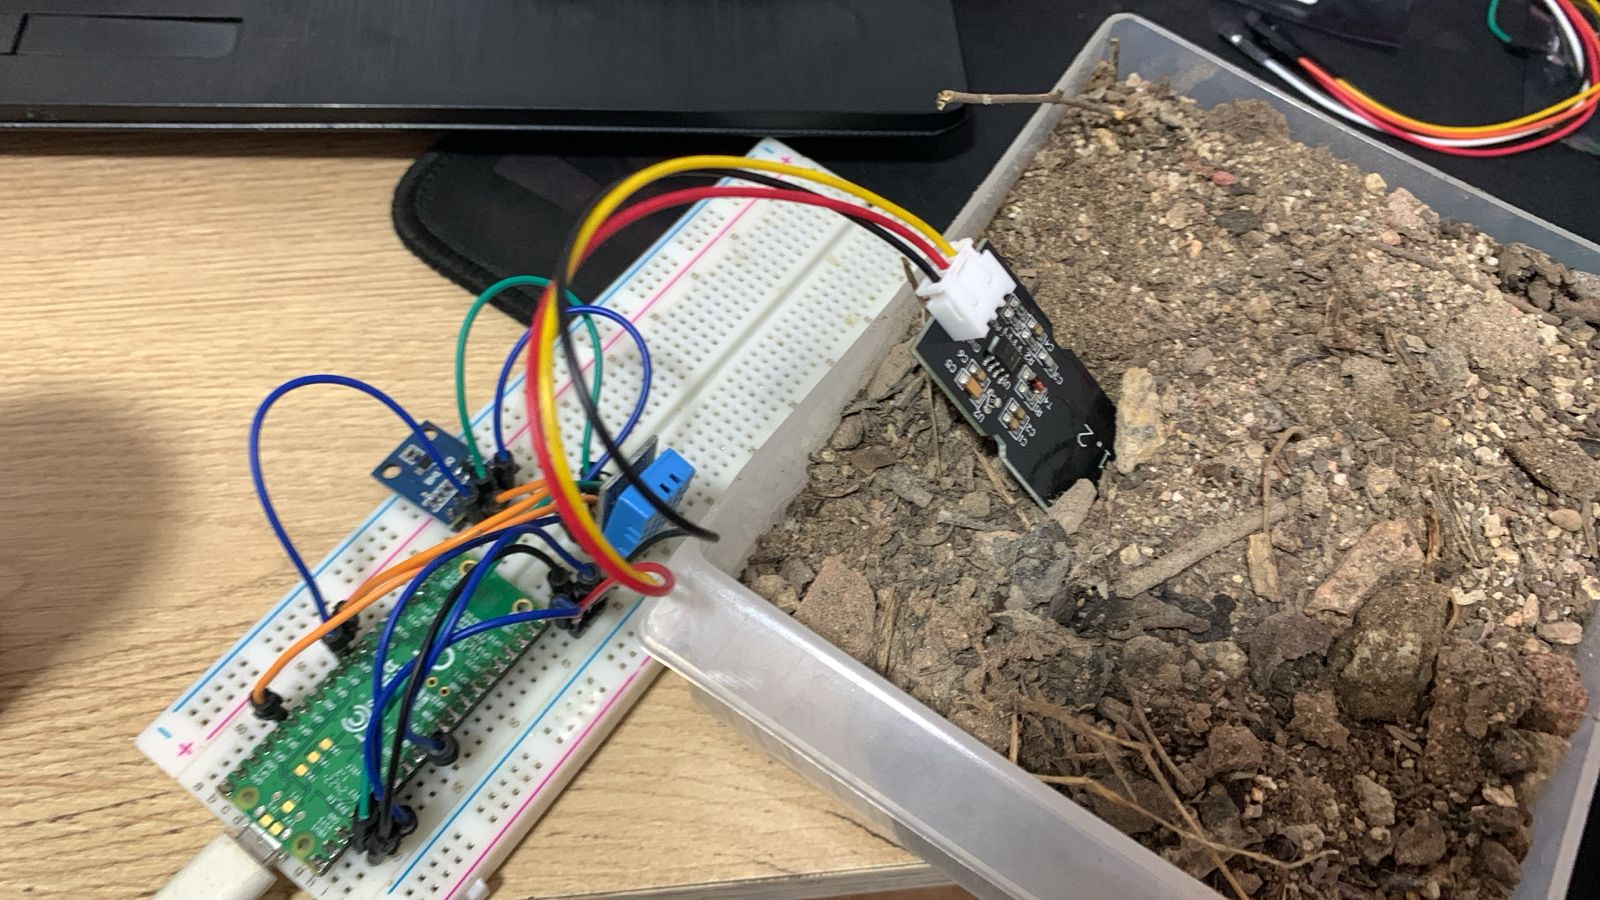
\includegraphics[width=0.7\textwidth]{img/fotos/sensorHumedadSuelo.png}
\caption{Sensor de humedad de suelo operativo.}
\end{figure}

Los valores en tiempo real se pueden ver en la pantalla oled con sus respectivas unidades.

\begin{figure}[h]
\centering
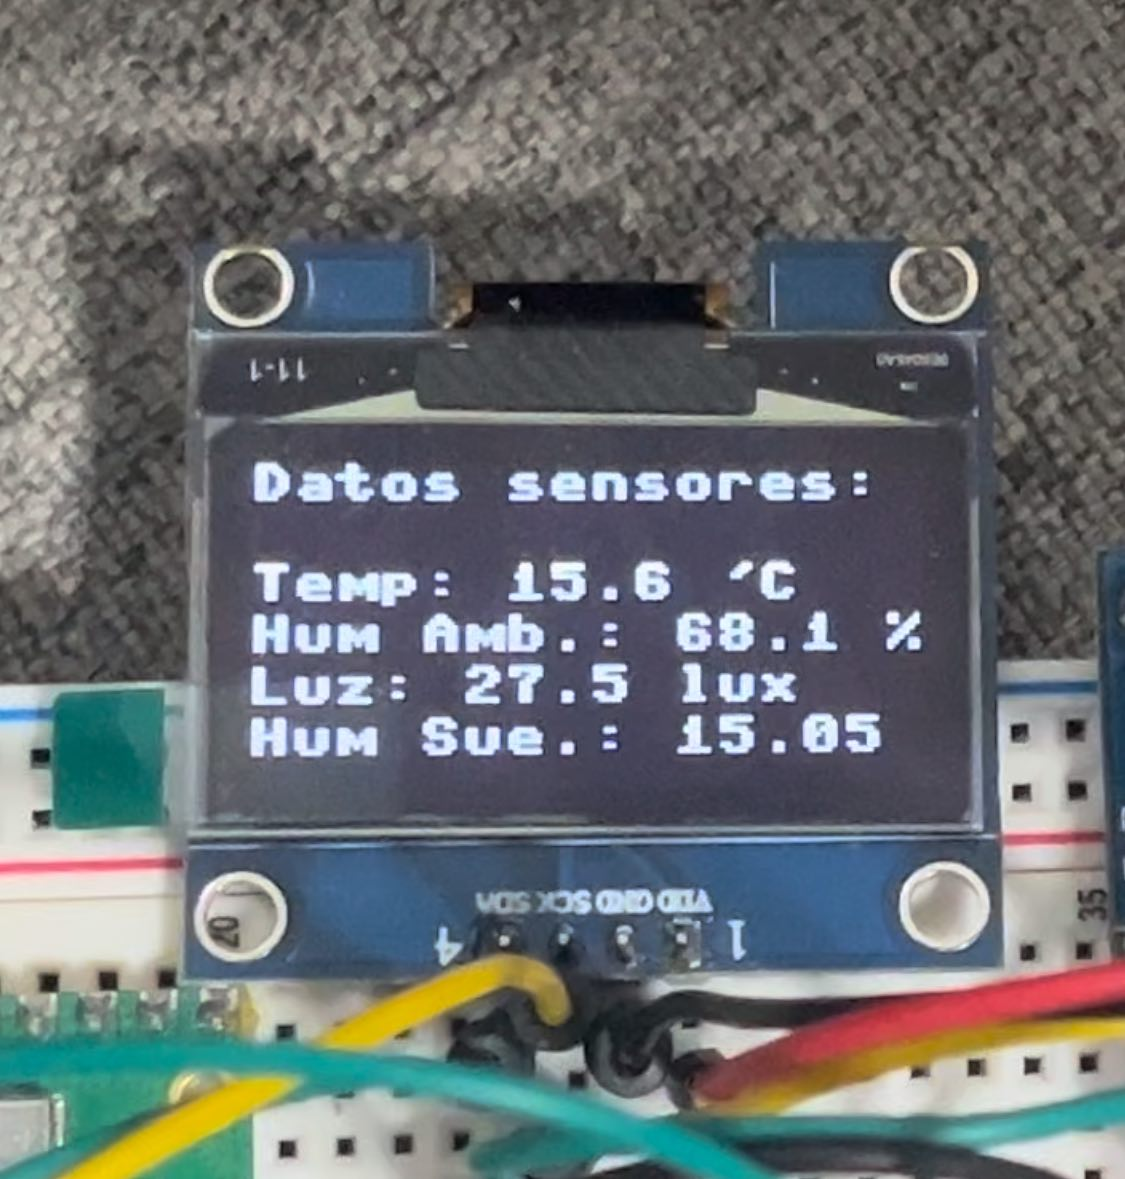
\includegraphics[width=0.71\textwidth]{img/fotos/oled1.png}
\caption{Pantalla oled mostrando los datos.}
\end{figure}

\subsection{InverIoT}

\begin{figure}[h]
\centering
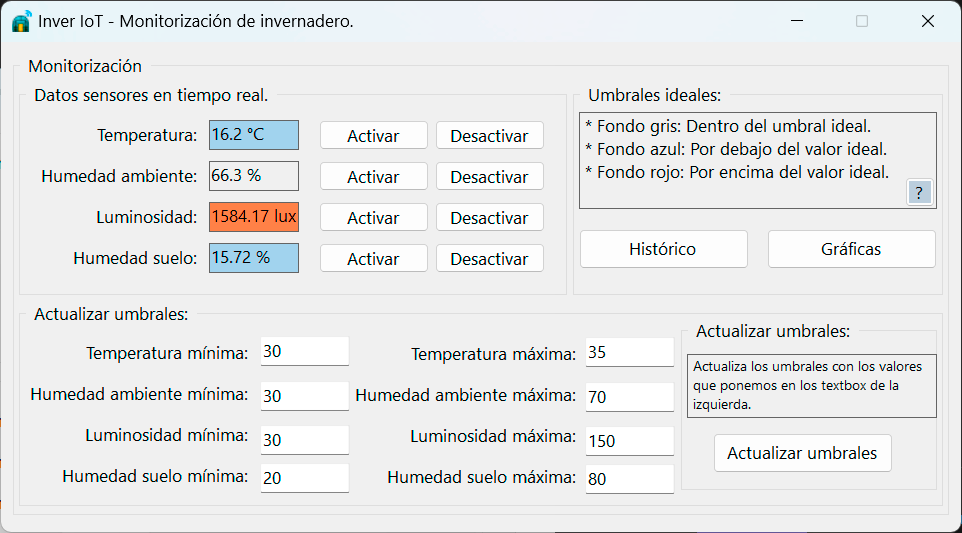
\includegraphics[width=1\textwidth]{img/desarrollo/InverIoT_Desktop.png}
\caption{Interfaz de la aplicación de escritorio.}
\end{figure}

La interfaz permite modificar los umbrales, tiene una comunicación bidireccional con la base de datos.

\begin{figure}[h]
\centering
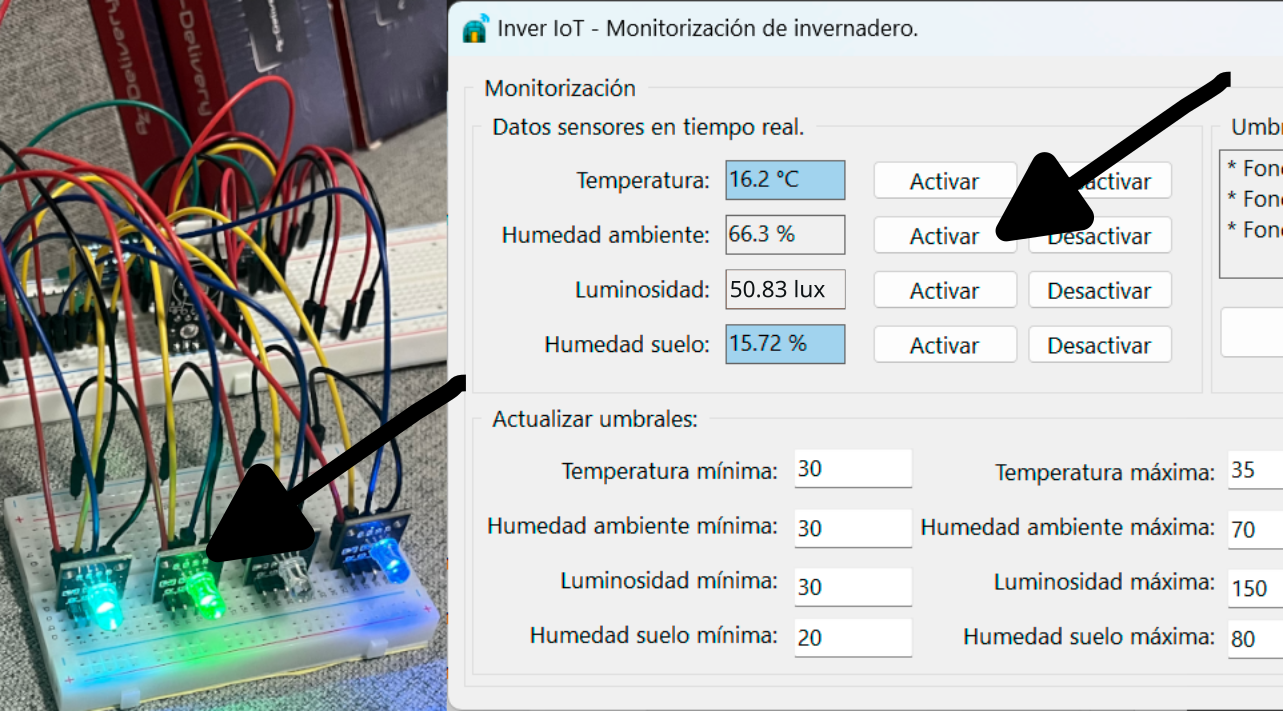
\includegraphics[width=1\textwidth]{img/desarrollo/InverIoT_verde_clickMecanismo.png}
\caption{Activación de mecanismo con un clic.}
\end{figure}

La activación del mecanismo está representado por el led verde prendido, pero si se desea activar otro mecanismo, solo desconectar del módulo led RGB el cable asociado al color verde, y conectarlo al mecanismo que se desea. Hacer esto solo si el nuevo mecanismo a activar es compatible en cuanto al voltaje necesario.


\begin{figure}[h]
\centering
\includegraphics[width=0.9\textwidth]{img/desarrollo/InverIoT_Histórico.png}
\caption{Accesso al histórico de datos.}
\end{figure}

\begin{figure}[h]
\centering
\includegraphics[width=1\textwidth]{img/desarrollo/InverIoT_Gráficas.png}
\caption{Capacidad de mostrar gráficas en un rango de fechas.}
\end{figure}

\subsection{dashboard}
Solo permite visualizar los datos, no envía comandos.

\begin{figure}[h]
\centering
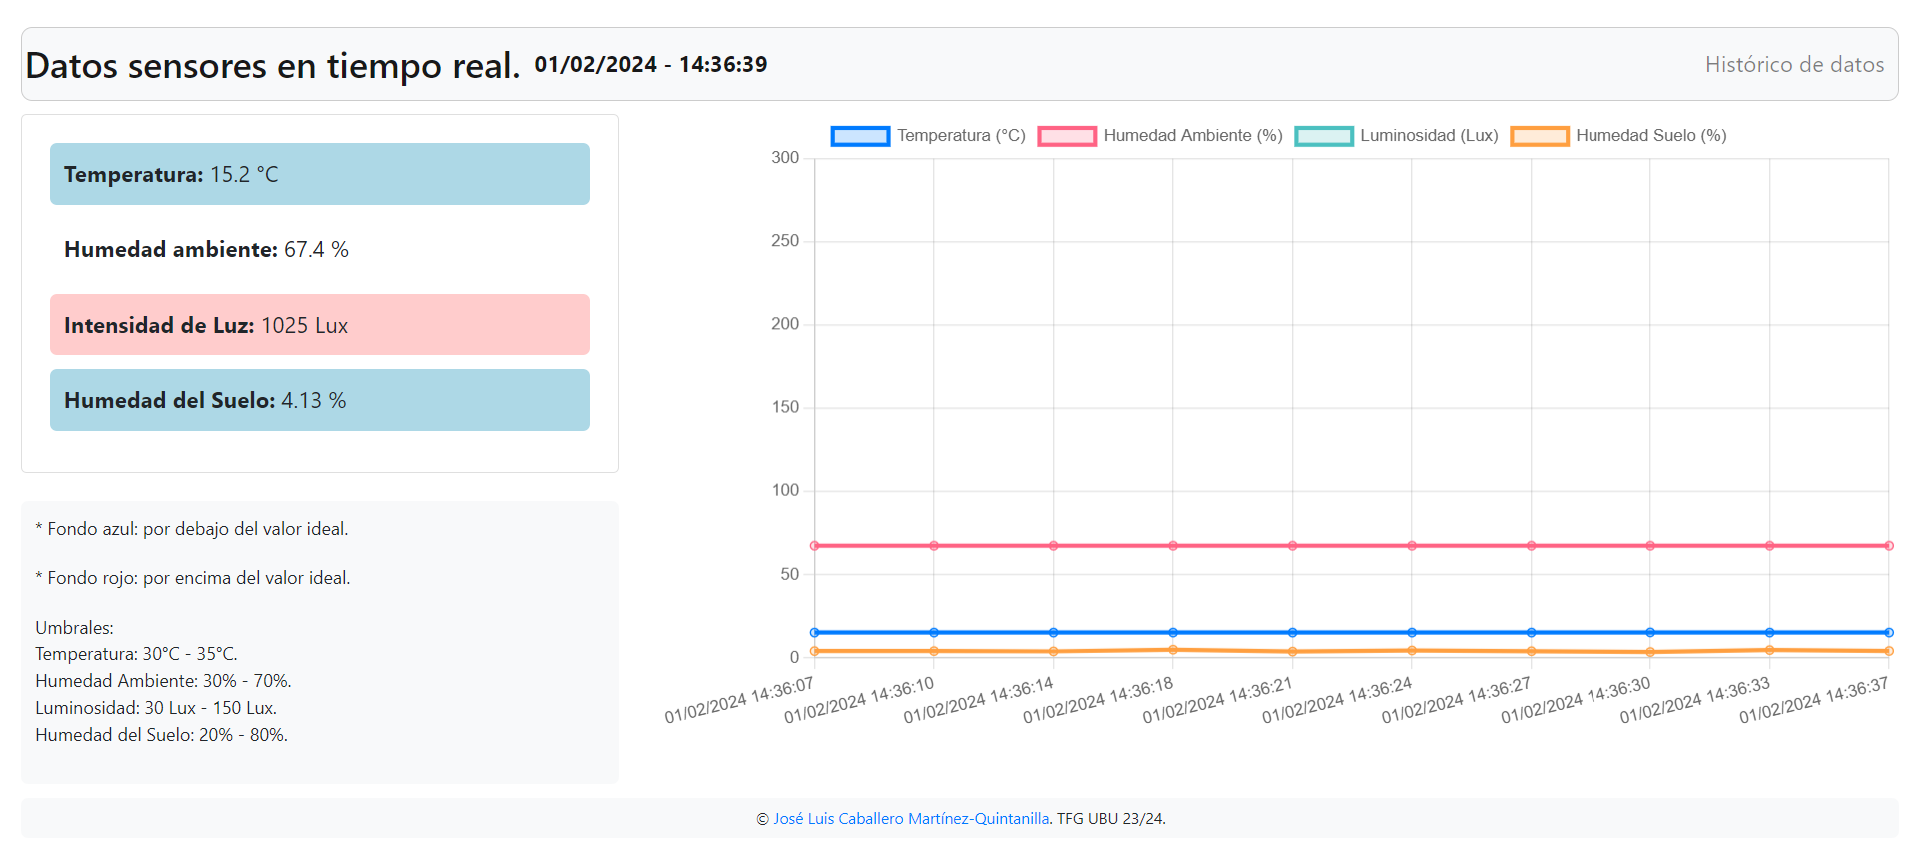
\includegraphics[width=1\textwidth]{img/desarrollo/Dashboard1.png}
\caption{El color rojo indica se ha sobrepasado el umbral.}
\end{figure}

\begin{figure}[h]
\centering
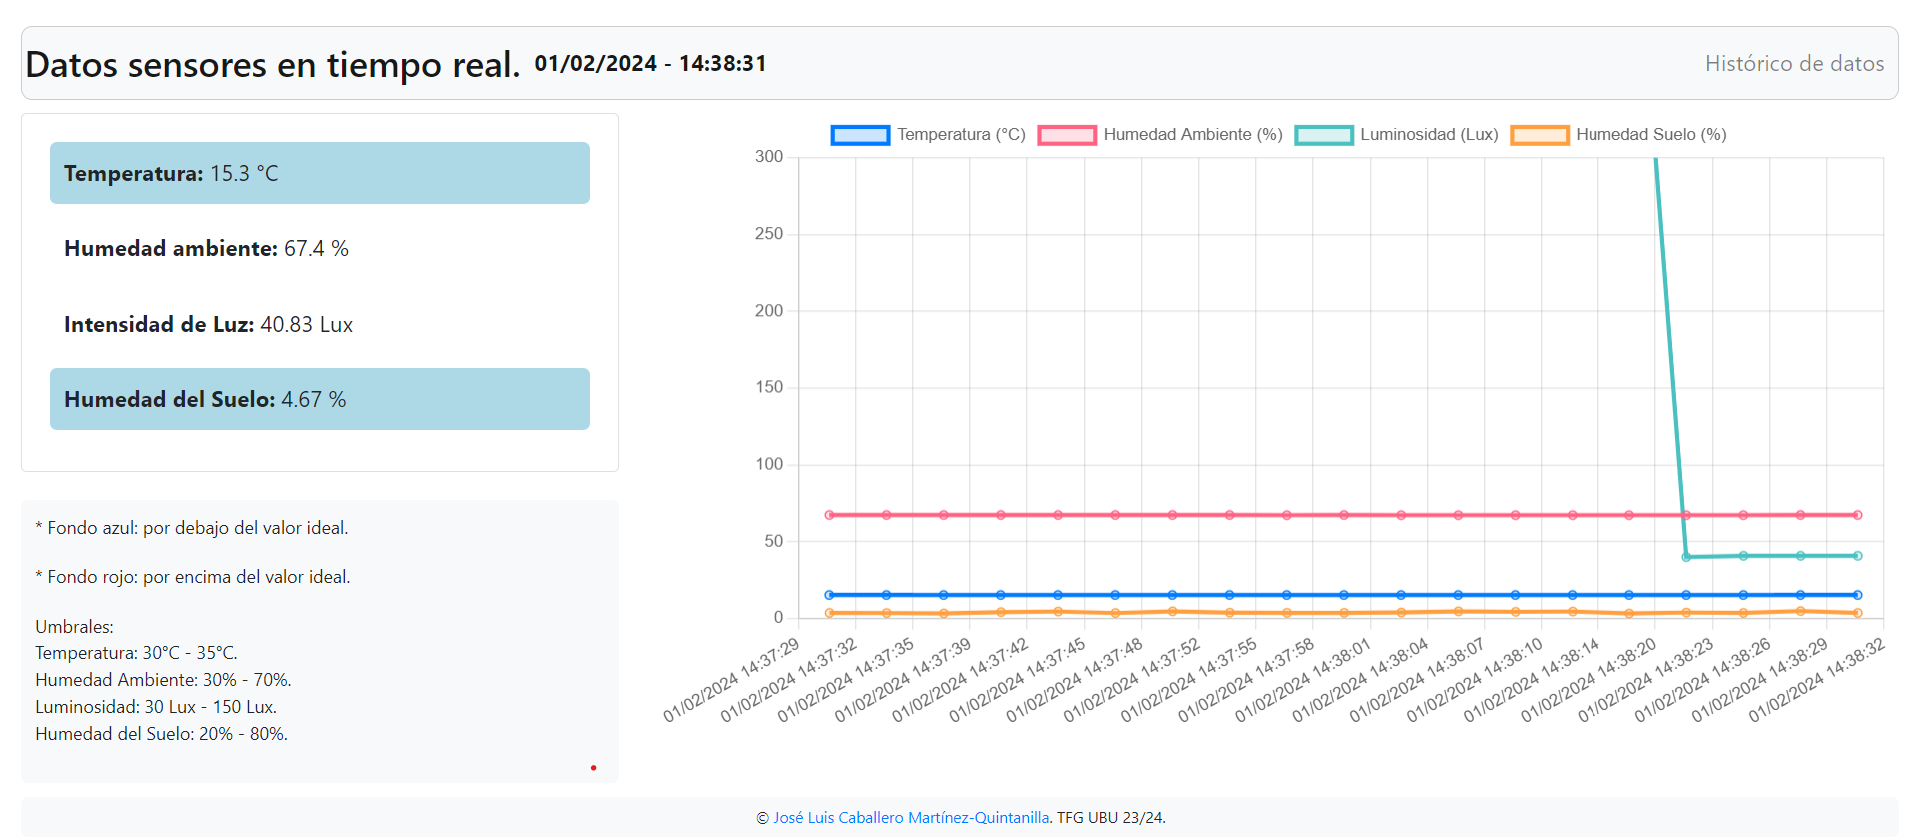
\includegraphics[width=1\textwidth]{img/desarrollo/Dashboard2.png}
\caption{El color azul indica está por debajo del umbral.}
\end{figure}

\subsection{Bot de telegram}
Permite enviar comandos y recibir alertas.

\begin{figure}[h]
\centering
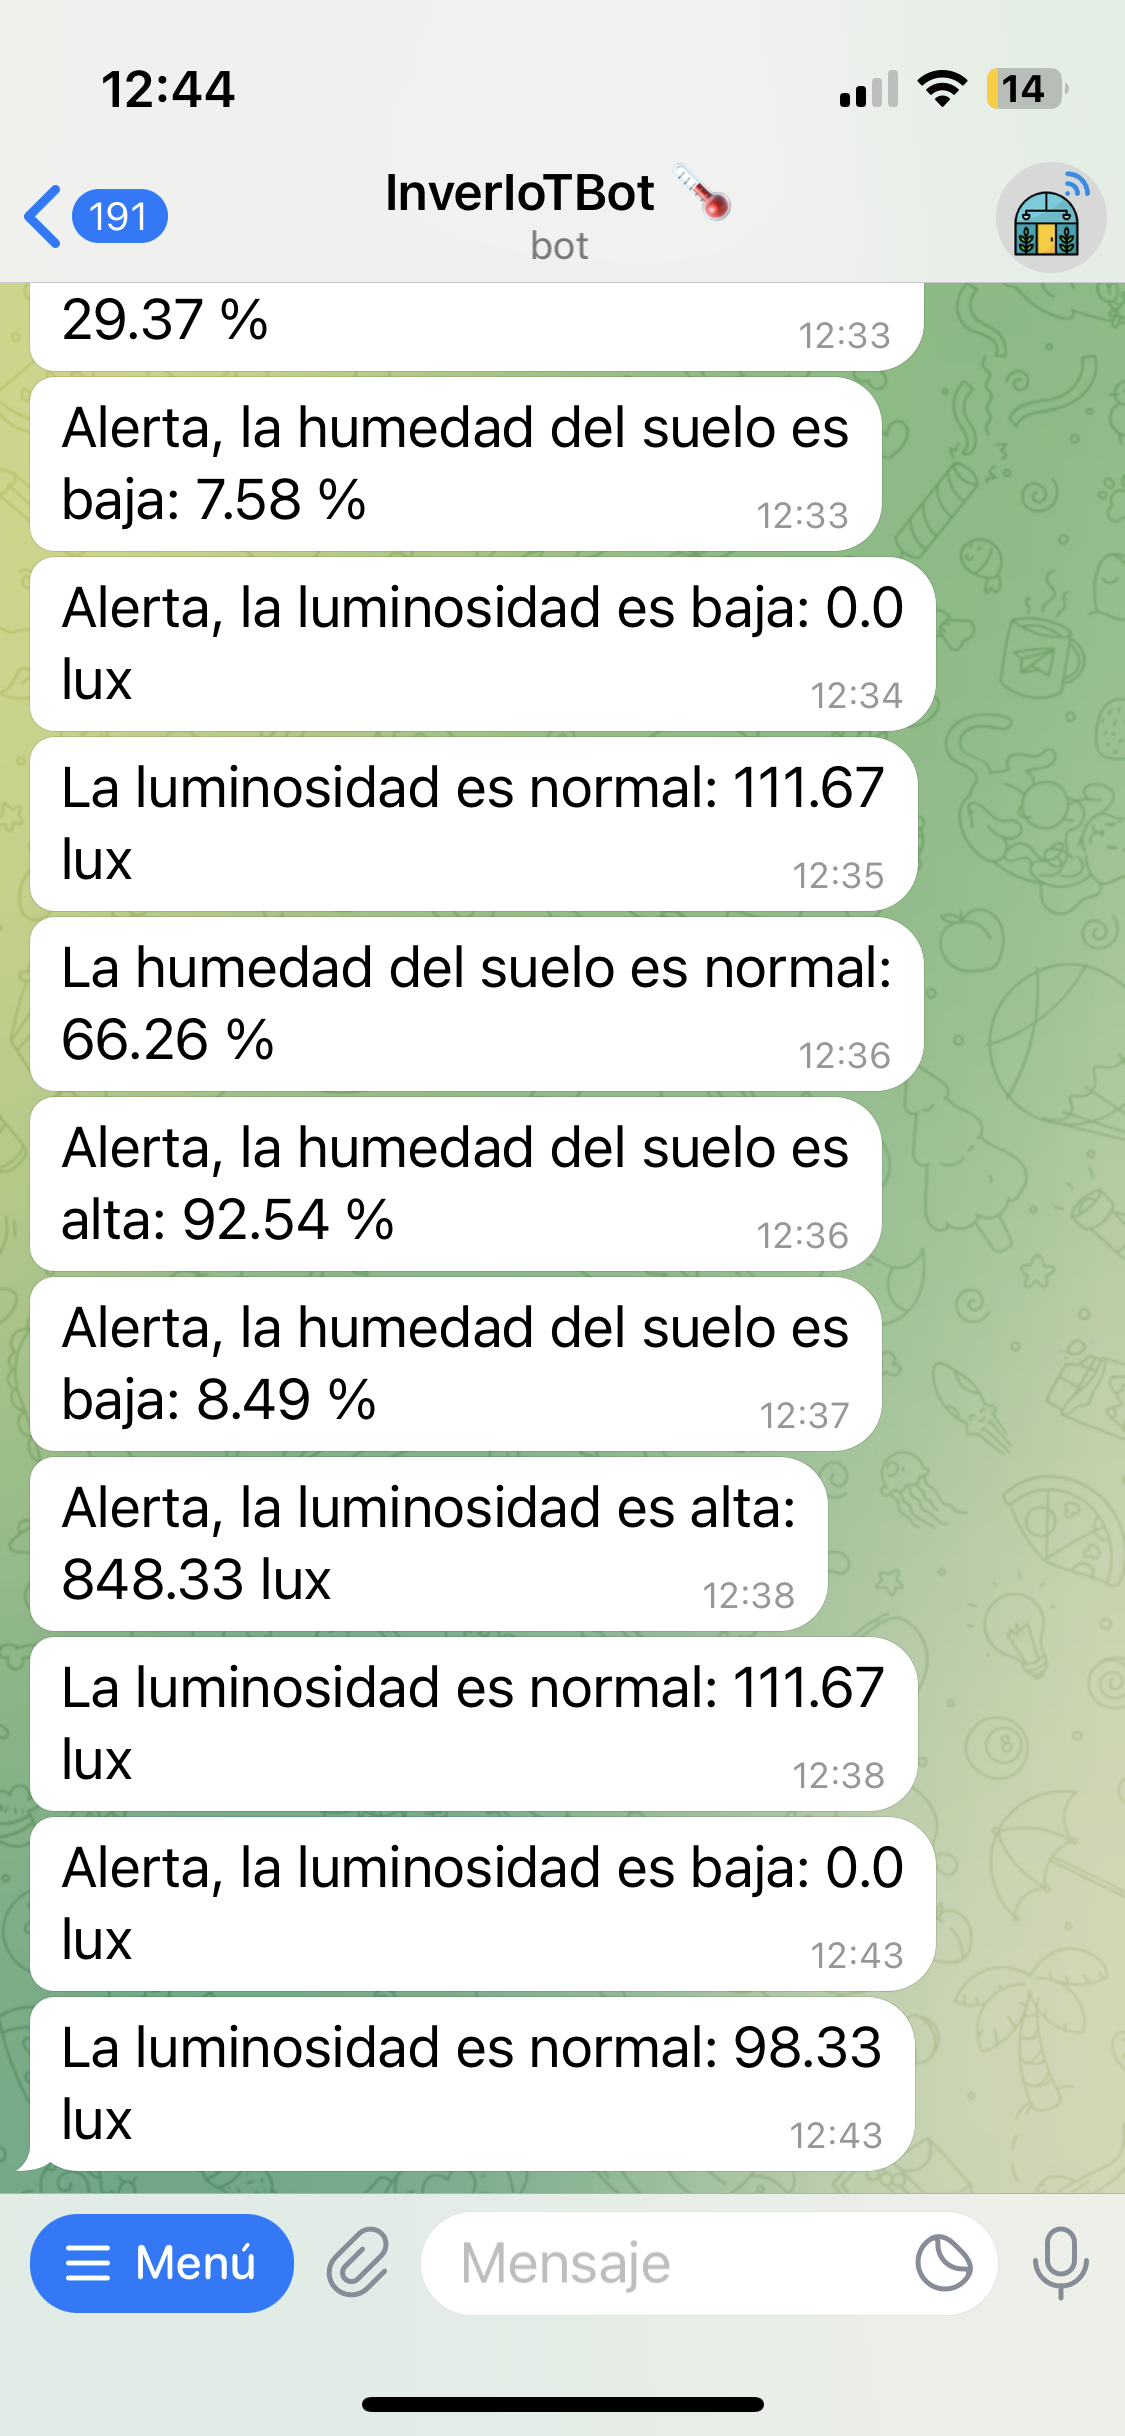
\includegraphics[width=0.7\textwidth]{img/desarrollo/BotTelegram_alertas.png}
\caption{Alertas recibidas por el bot de Telegram.}
\end{figure}

\begin{figure}[h]
\centering
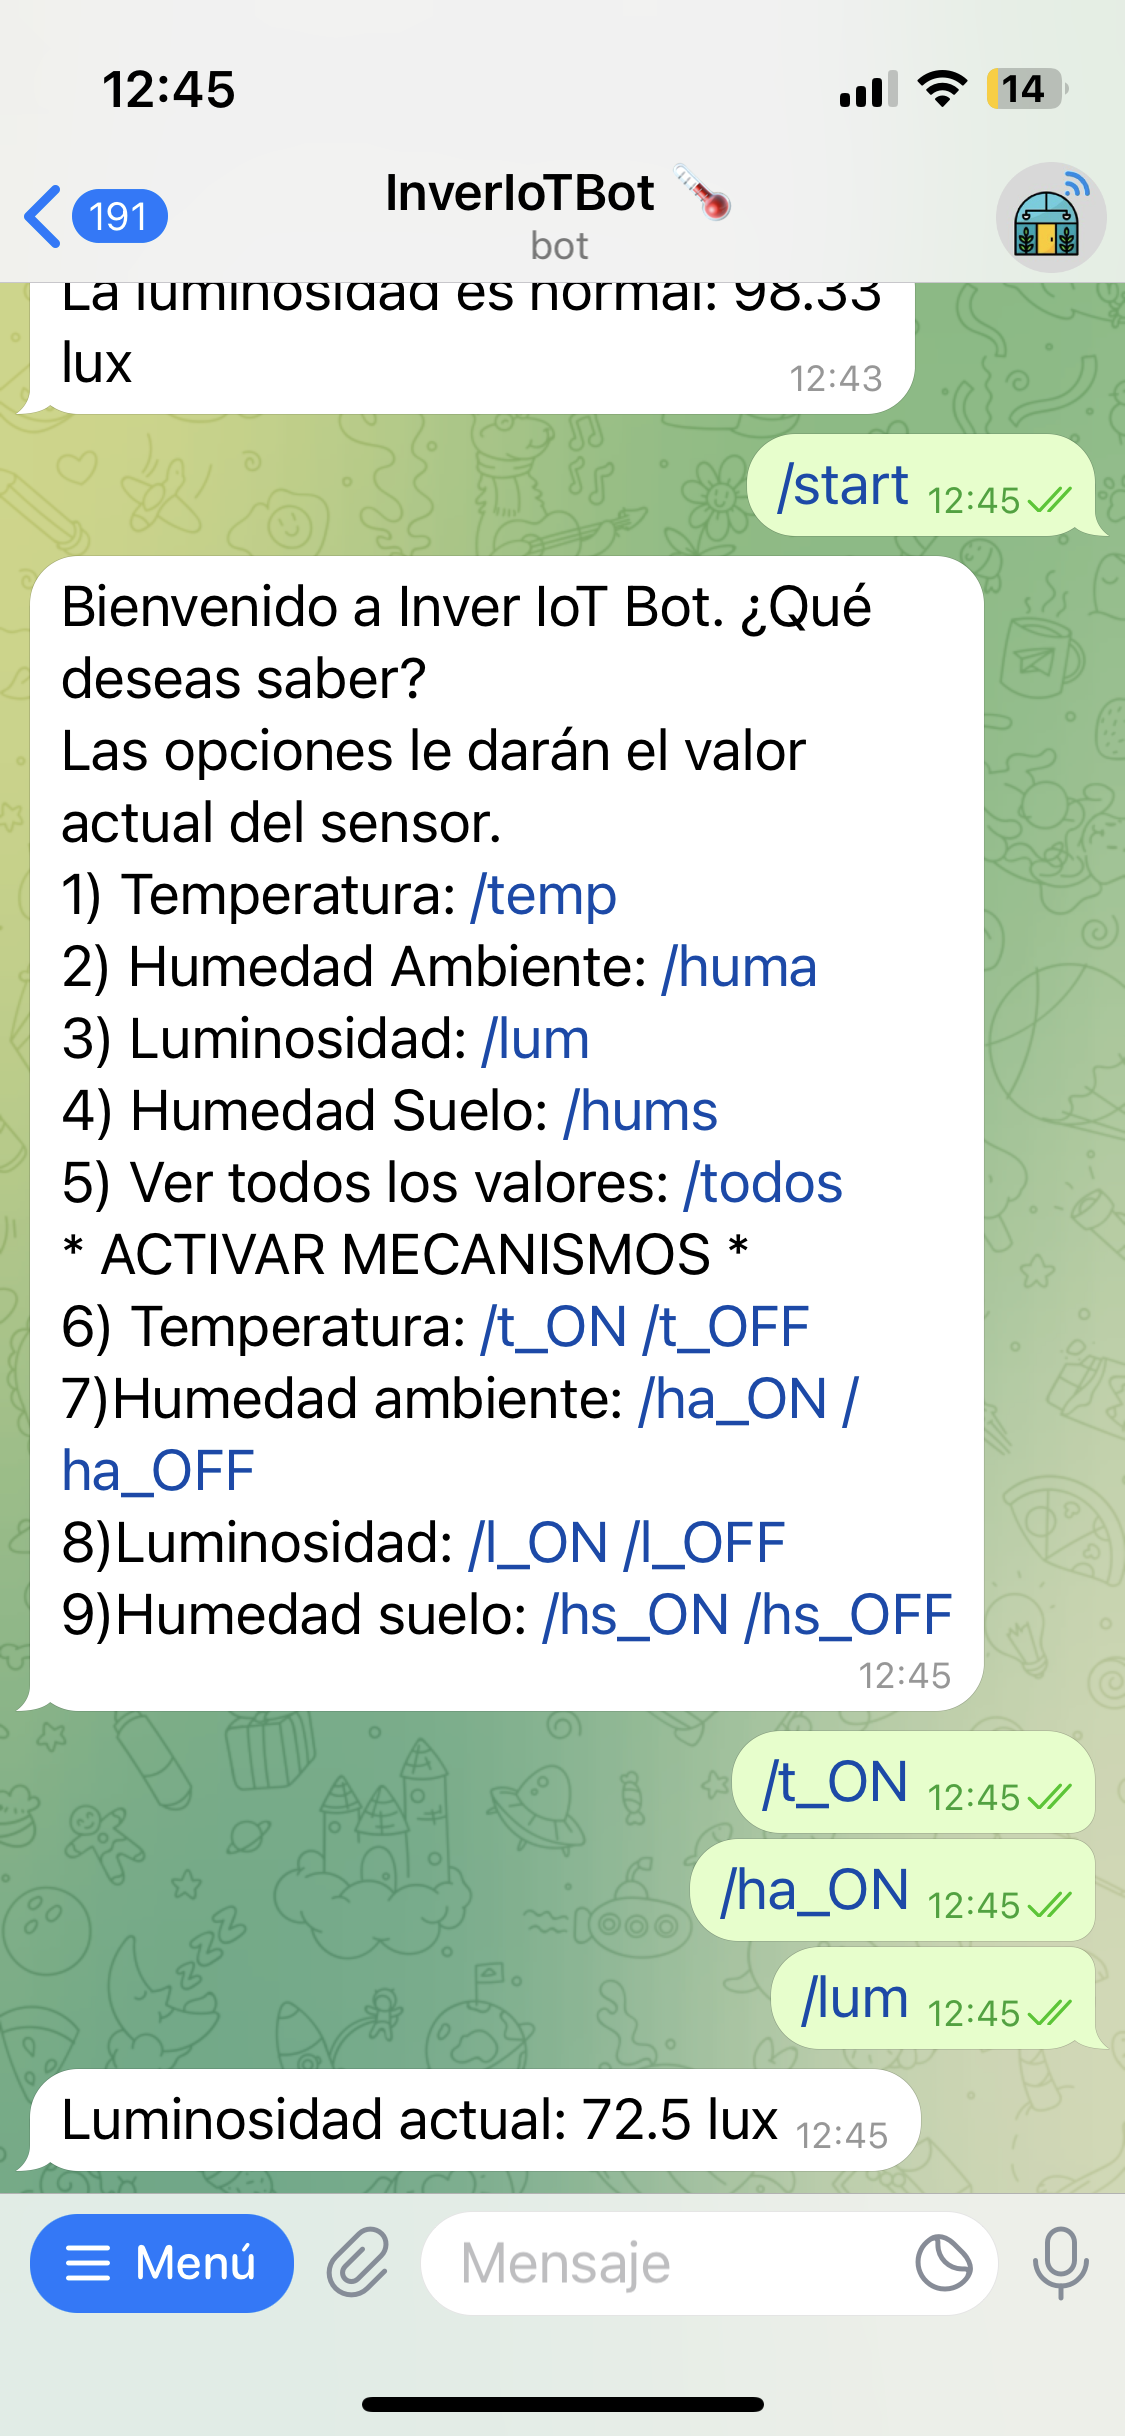
\includegraphics[width=0.7\textwidth]{img/desarrollo/BotTelegram_comandos.png}
\caption{Capacidad de enviar comandos desde Telegram.}
\end{figure}
